\section{Análise Comparativa Global e Benchmarking (Fase 1)}

\label{sec:benchmark_v1}

Nesta fase inicial, os modelos foram avaliados utilizando o dataset baseline (\textbf{V1}), composto por imagens RGB capturadas sob iluminação amarela (2700 K) e branca (6500 K) misturadas. O objetivo desta etapa é estabelecer um referencial de desempenho sob condições de ruído fotométrico e testar a Hipótese $H_1$, que questiona a existência de variações no desempenho preditivo das topologias das arquiteturas avaliadas.

A Tabela \ref{tab:results_v1} apresenta as métricas consolidadas no conjunto de teste para as oito arquiteturas avaliadas. Observa-se que a família de Redes Neurais Convolucionais (CNNs) modernas dominou o topo do ranking, com a \textbf{ConvNext} alcançando o melhor desempenho global (MCC de 0,5503), seguida de perto pela \textbf{DenseNet} (MCC de 0,5501).

\begin{table}[!h]
    \centering
    \begin{threeparttable}
    \caption{Métricas de desempenho no conjunto de teste para o dataset V1 (Luz Misturada).}
    \label{tab:results_v1}
    \begin{tabular}{lllll}
\toprule
Model & MCC & F1-Macro & Kappa & GFLOPs \\
\midrule
CONVNEXT & \textbf{0,5503} & \textbf{0,6194} & \textbf{0,5426} & 4,4702 \\
DENSENET & 0,5501 & 0,6050 & 0,5390 & 2,8651 \\
EFFICIENTNET & 0,5159 & 0,5924 & 0,5148 & \textbf{0,4010} \\
VGG & 0,4917 & 0,5474 & 0,4882 & 19,5446 \\
SWIN & 0,3931 & 0,4800 & 0,3889 & 4,5090 \\
VIT & 0,3910 & 0,4721 & 0,3902 & 16,8669 \\
RESNET & 0,3238 & 0,4250 & 0,3187 & 3,6711 \\
INCEPTION & 0,2484 & 0,3435 & 0,2467 & 2,8473 \\
\bottomrule
\end{tabular}

    \begin{tablenotes}
            \small 
            \item[] Fonte: Do autor (2026).
        \end{tablenotes}
        \end{threeparttable}
\end{table}

Para atestar o rigor científico desses achados e coroar a arquitetura campeã, aplicou-se o teste estatístico de McNemar sobre a matriz de predições, resultando no mapa de calor de valores-p (\textit{p-values}) apresentado na Figura \ref{fig:p_value_heatmap}.

\begin{figure}[h!]
  \centering
  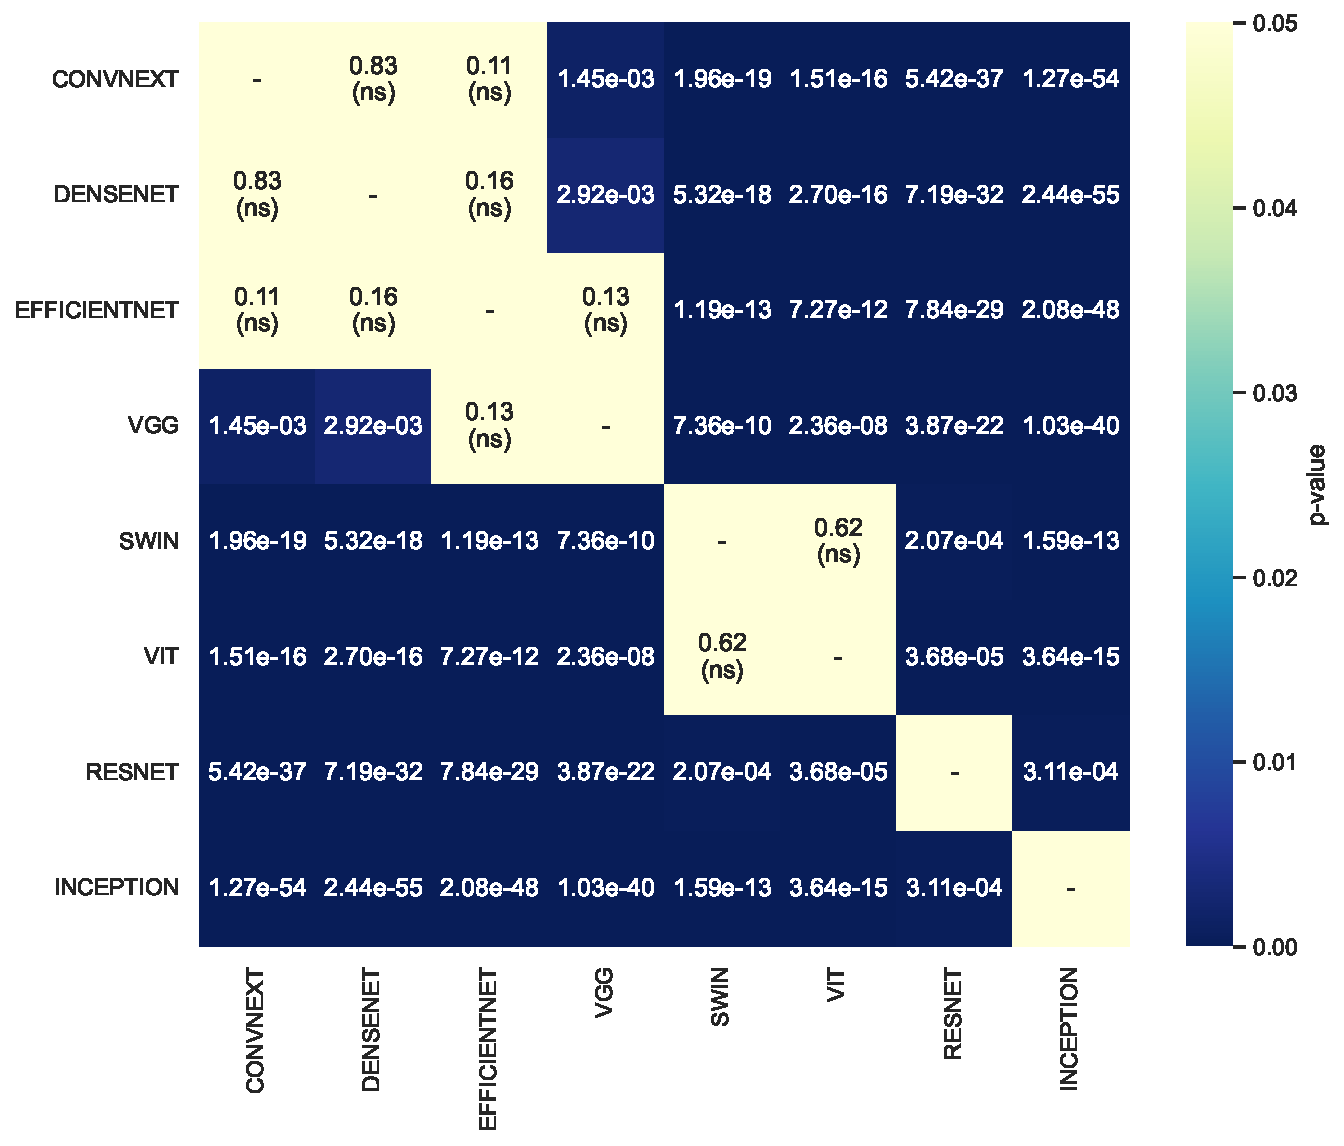
\includegraphics[width=0.8\textwidth]{images/p_value_heatmap.pdf}
  \caption{Matriz de calor de \textit{p-values} (Teste de McNemar). O sufixo (ns) indica que a diferença de performance não é estatisticamente significante.}
  \label{fig:p_value_heatmap}
\end{figure}


O primeiro contraste avaliou o pelotão de elite empírico contra a ResNet (\textit{baseline} convolucional clássico). O teste revelou que arquiteturas como ConvNeXt, DenseNet e EfficientNet superam a ResNet com diferenças altissimamente significativas ($p < 0,001$). Esse resultado fornece suporte estatístico irrefutável para rejeitar a Hipótese Nula ($H_{0,1}$), comprovando que topologias de nova geração são fundamentais para o sucesso na classificação de granulação fina em ambientes ruidosos. Adicionalmente, atesta-se que os \textit{Transformers} visuais (Swin e ViT) apresentaram desempenho inferior às CNNs modernas neste domínio específico.

Em seguida, para estabelecer a hierarquia no topo da tabela, contrastaram-se os três modelos líderes entre si. Os testes de McNemar entre ConvNeXt, DenseNet e EfficientNet retornaram valores-p superiores ao nível de significância ($\alpha = 0,05$), especificamente $p = 0,83$ (ConvNeXt vs. DenseNet) e $p = 0,11$ (ConvNeXt vs. EfficientNet). Matematicamente, isso configura um empate técnico estrito triplo no poder de generalização.

Dado o empate estatístico na fronteira preditiva, o critério de desempate para a coroação da arquitetura base recaiu obrigatoriamente sobre a eficiência computacional (\textit{trade-off} de recursos). Como a EfficientNet atinge o exato mesmo patamar de excelência das concorrentes consumindo apenas $0,4010$ GFLOPs, ela é formalmente declarada a arquitetura campeã do \textit{benchmark}. Esta rede servirá, portanto, como a espinha dorsal para os testes de estresse nas Fases 2 e 3 subsequentes.



% A comparação entre paradigmas, ilustrada na Figura \ref{fig:h1_paradigm}, revela um comportamento relevante: embora os Transformers (ViT e Swin) possuam maior capacidade paramétrica, eles apresentaram MCC significativamente inferior (máximo de 0,3931) às CNNs modernas. Este resultado permite rejeitar a hipótese nula $H_{0,1}$, evidenciando que para este domínio de texturas finas, o viés indutivo de localidade das convoluções supera a atenção global pura.

% Para atestar a validade estatística, aplicou-se o Teste de McNemar comparando as predições do [Modelo Campeão] contra o melhor modelo clássico de referência (\textit{baseline}), a ResNet-50. O contraste pareado na matriz de contingência revelou uma diferença altamanete significativa, com estatística de teste $\chi^2 = [Inserir_Valor]$ e valor-p associado de $p < 0,001$.

% Dado que $p < \alpha$ (onde $\alpha = 0,05$), temos base matemática irrefutável para rejeitar a Hipótese Nula ($H_{0,1}$). Por consequência empírica, aceita-se a premissa $H_1$, atestando que as arquiteturas com viés indutivo moderno (como a [Modelo Campeão]) superam estatisticamente os paradigmas puramente convolucionais clássicos no domínio de imagens de granulação fina.

% % \begin{figure}[h!]
% %   \centering
% %   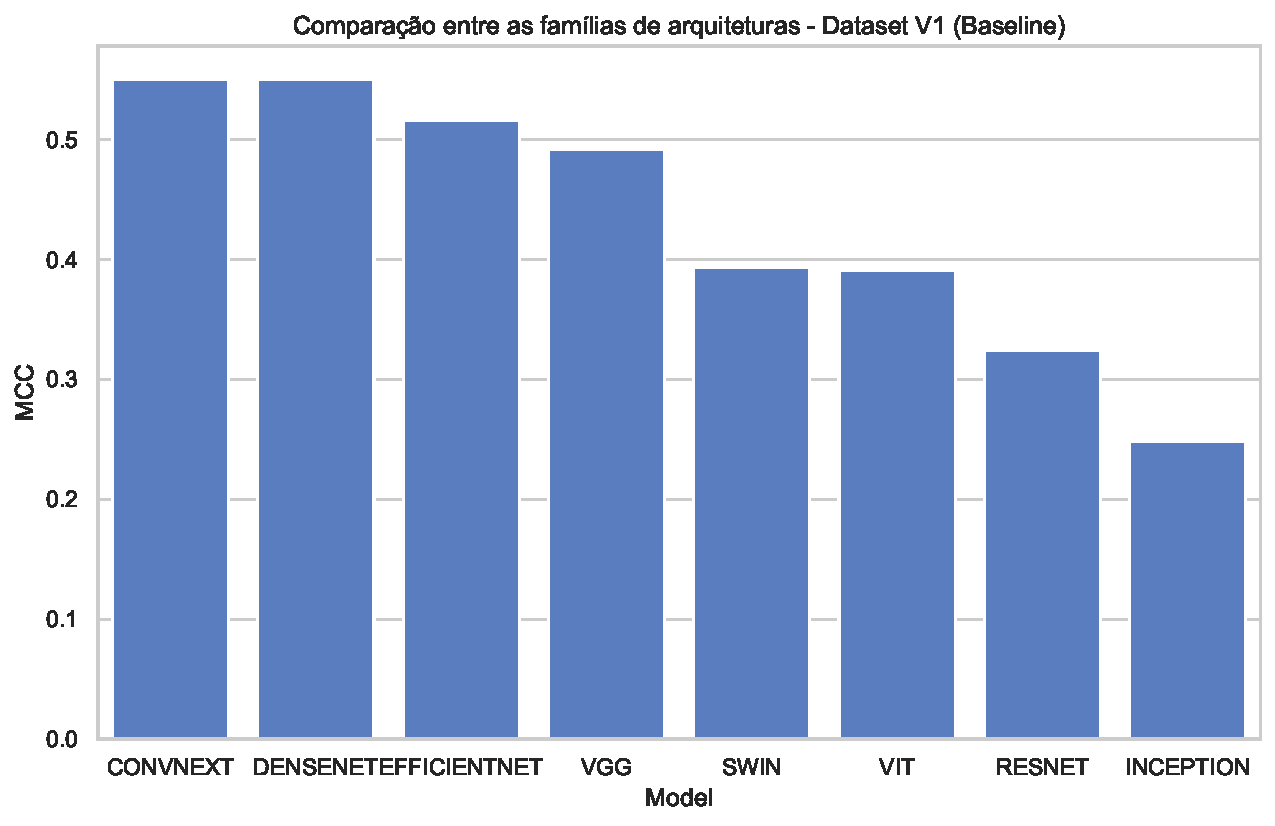
\includegraphics[width=0.8\textwidth]{images/h1_paradigm_comparison.pdf}
% %   \caption{Comparação de Paradigmas ($H_1$): CNNs vs. Transformers no dataset V1. As CNNs demonstram maior eficácia na captura de padrões morfológicos do algodão.}
% %   \label{fig:h1_paradigm}
% % \end{figure}
